\documentclass[a4paper,12pt]{article}

\input{packages}

\begin{document}

\pagebreak
\subsection{Théorème de l'intersection des hauteurs}
\begin{theorem}
Les hauteurs d'un triangle concourent en un seul point nommé orthocentre.
\end{theorem}

\begin{proof}
Nous considérons le triangle quelconque $ABC$, ayant $h_A$ comme hauteur passant $A$.

\begin{figure}[H]
        \centering
        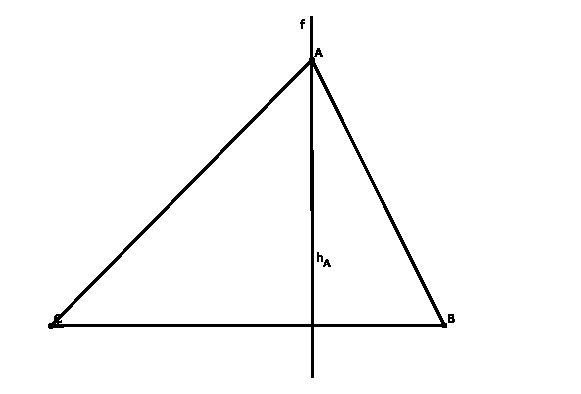
\includegraphics[scale=1]{hauteur1.eps}
    \end{figure}
    
    
\begin{hyp}
$\triangle ABC$ est quelconque
\end{hyp}
\begin{concl}
les hauteurs de $\triangle ABC$ concourent en un seul point
\end{concl}
Nous construisons les points $D$, $E$ et $F$ ainsi que:
\begin{itemize}
    \item $DE \parallel CB$
    \item $EF \parallel CA$
    \item $DF \parallel AB$
\end{itemize}

\begin{figure}[H]
        \centering
        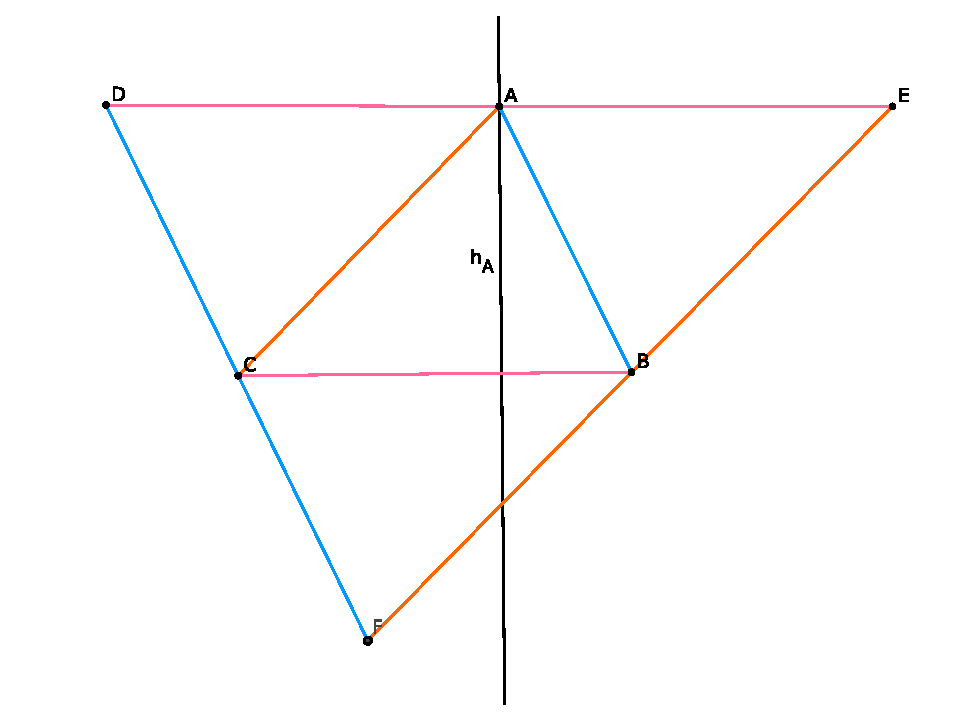
\includegraphics[scale=0.7]{hauteur2.eps}
    \end{figure}
    
    
Dès lors, nous obtenons par construction deux parallélogrammes $AEBC$ et $DABC$ (ils ont deux paires de côtés parallèles). Cela implique que $AE \equiv CB$ et $DA \equiv CB$ (théorème \ref{th:parallelogramme}) et donc $AE \equiv DA$. 

\begin{figure}[H]
        \centering
        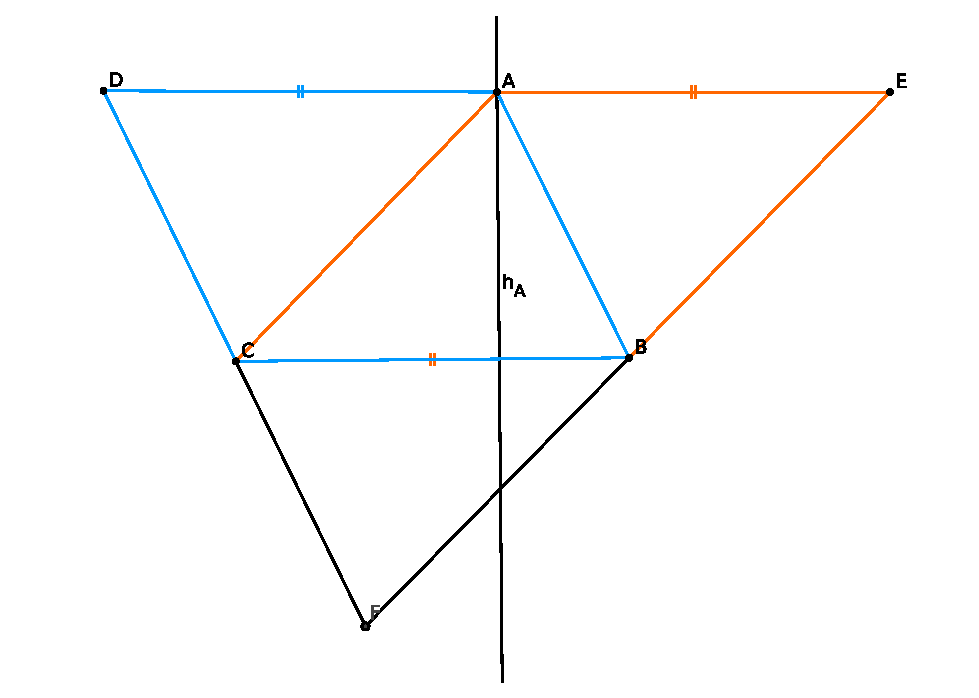
\includegraphics[scale=0.7]{hauteur3.eps}
    \end{figure}

Ainsi, $h_a$ est la médiatrice du segment $DE$, car elle le découpe en deux parties égales et qu'elle y est perpendiculaire. Les hauteurs du triangle $ABC$ sont donc les médiatrices du triangle $DEF$.

\begin{figure}[H]
        \centering
        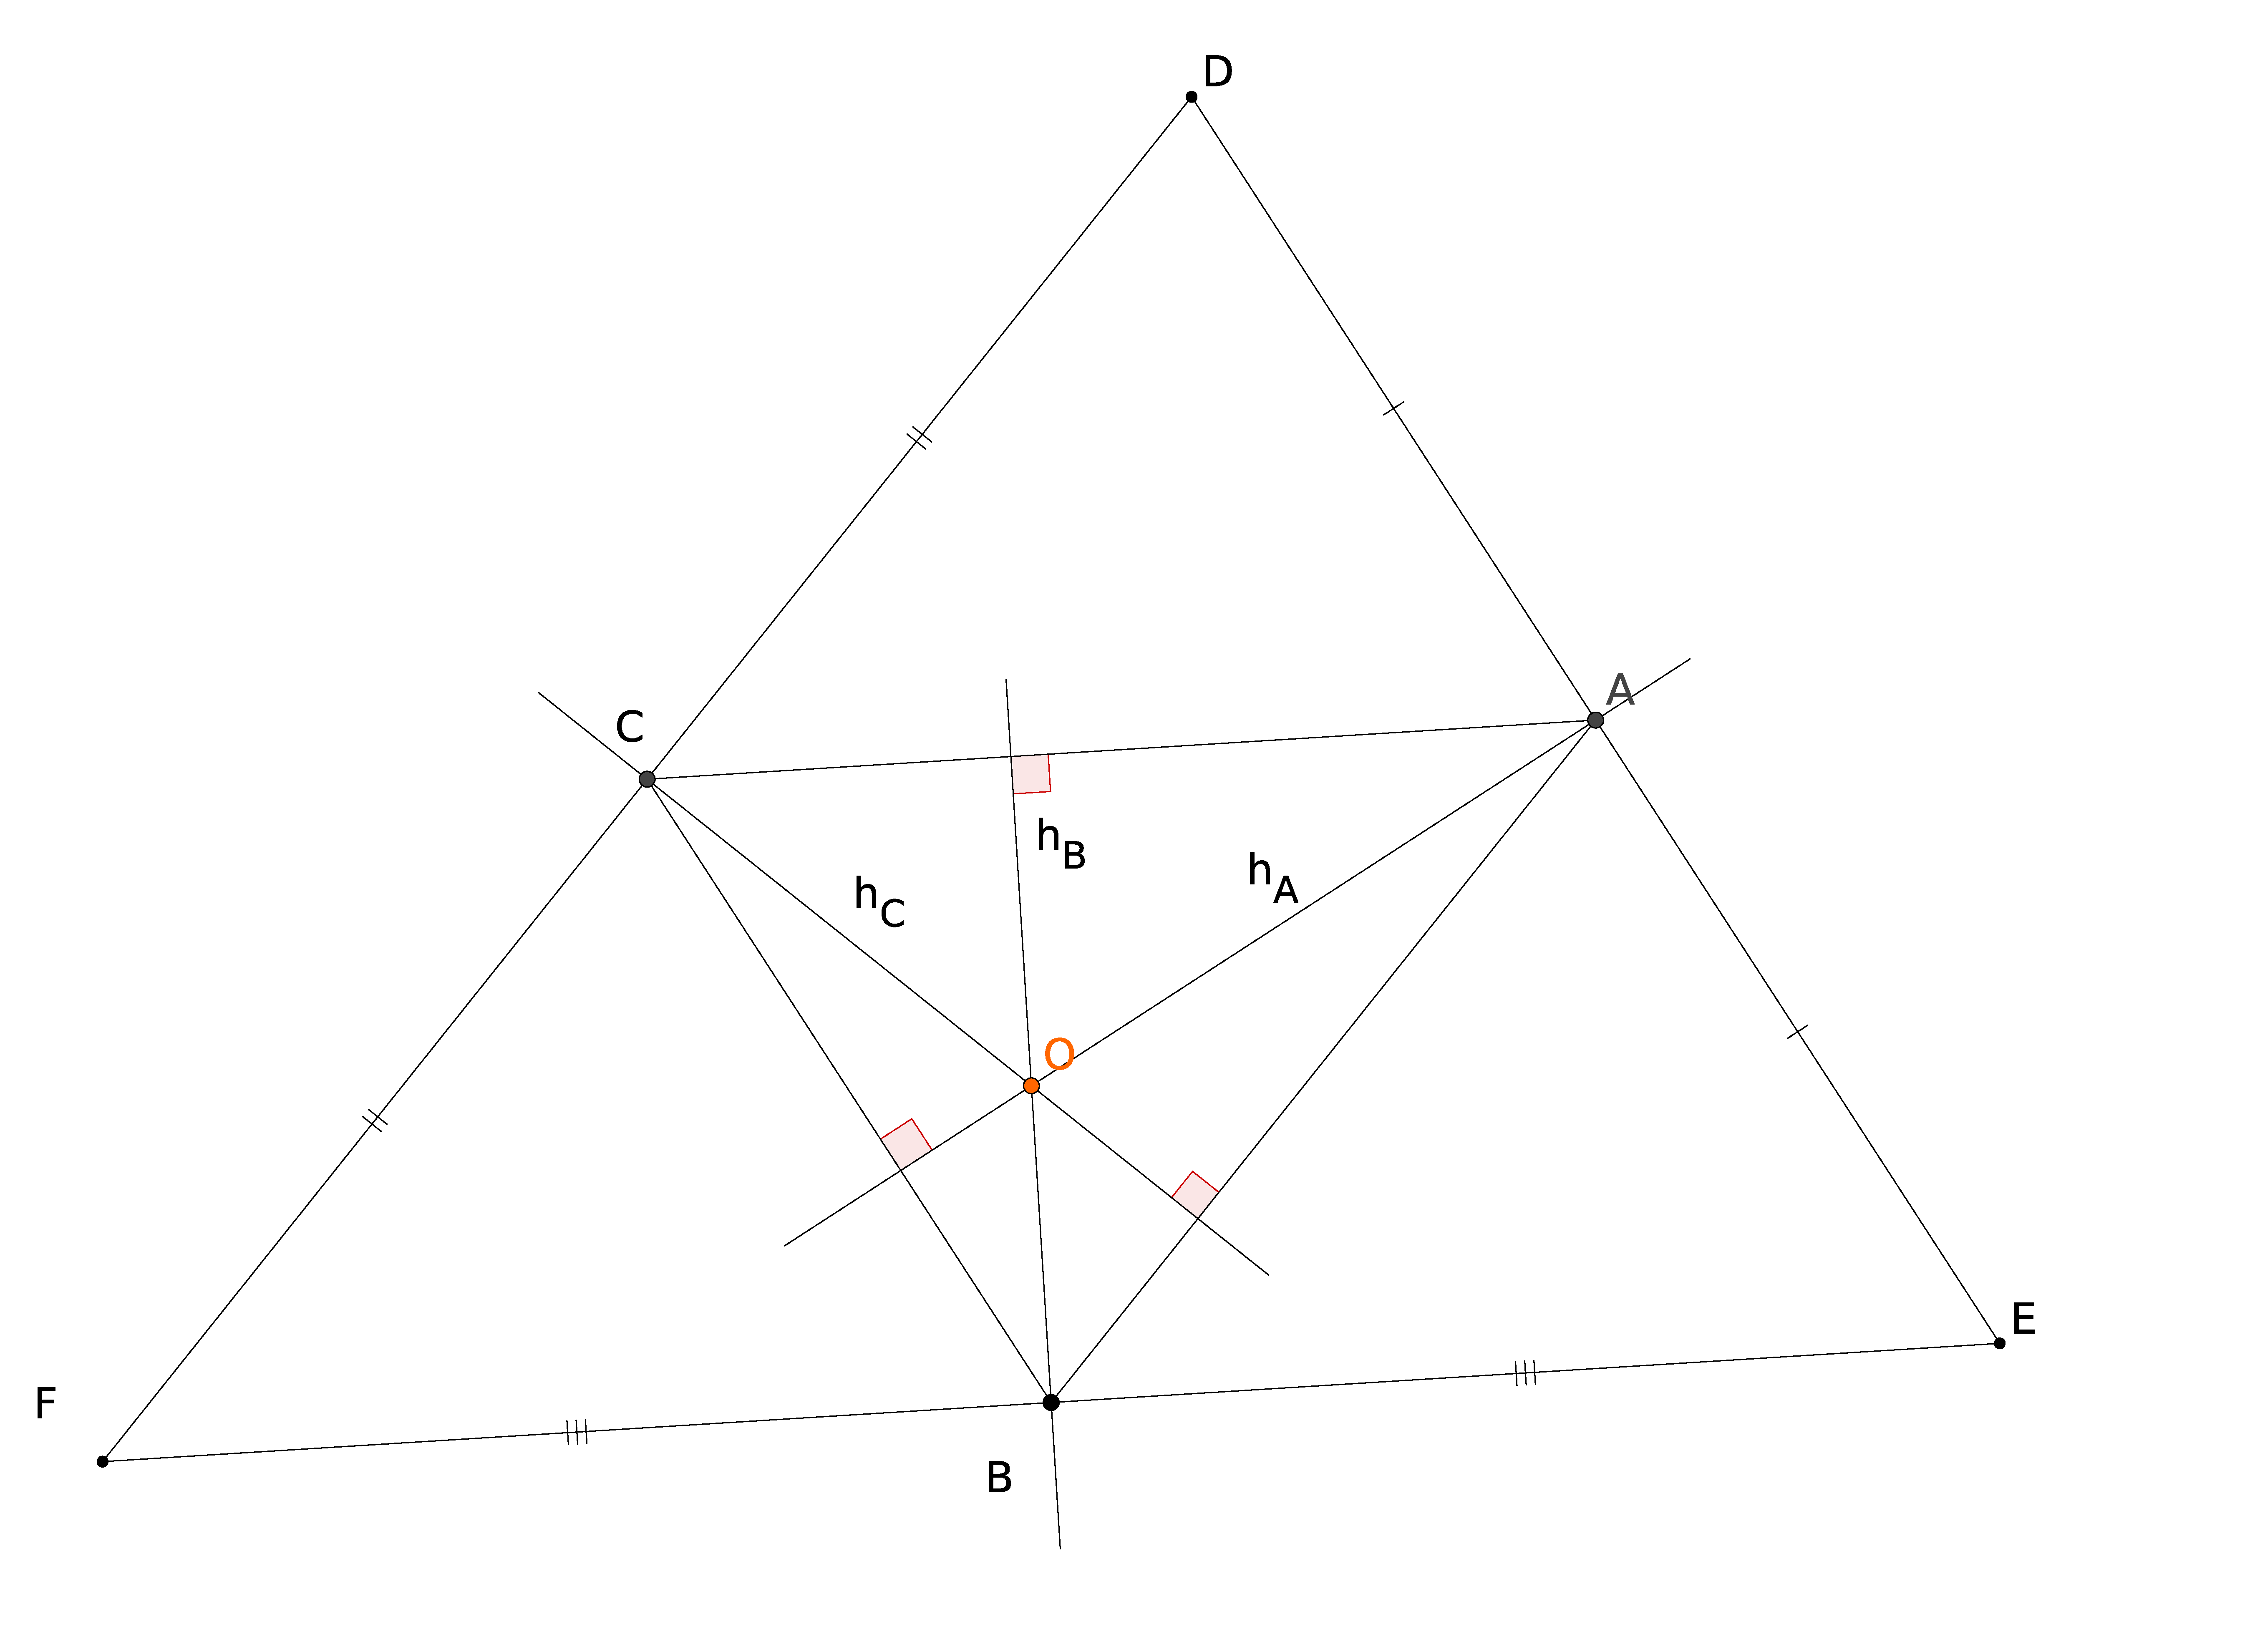
\includegraphics[scale=0.15]{hauteur4.eps}
    \end{figure}

Cela signifie que les hauteurs d'un triangle concourent en un point, car elles sont confondues avec les médiatrices d'un triangle augmenté, or nous avons démontré que les médiatrices d'un triangle s'intersectent en un seul point (corollaire \ref{cor:mediatrices}).
\end{proof}

\end{document}